%%%%%%%%%%%%%%%%%%%%
\newcommand{\functionANHTAO}[2]{
	\functionSignature{\texttt{anhtao-path}}{\varAtomicTask{}{}, \varAgent{}{}}
}

\subsection{Algorithm for optimising hierarchical task allocation in networks of agents}

The \acronymWSNOptimisationExtended{}{} algorithm is defined in Algorithms \ref{alg:wsn_optimisation_sink}
and \ref{alg:wsn_optimisation_arc}, which are split for clarity. The flowchart in Figure \ref{fig:algorithm-flow}(a) shows how sink node agents decompose composite tasks, choose actions to take, allocate atomic tasks, and return results. In Figure \ref{fig:algorithm-flow}(b) we can see how agents in a task-path choose actions, and how they execute or re-allocate the atomic tasks they have been allocated.

\begin{figure}[ht]
	\centering
	\begin{subfigure}{.49\textwidth}
		\centering
		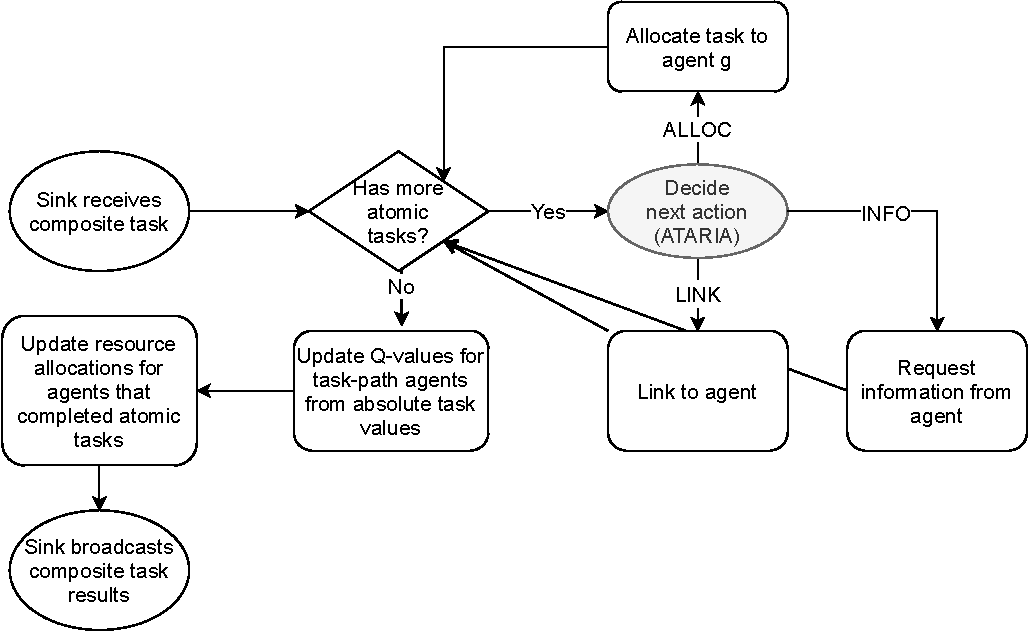
\includegraphics[width=0.9\linewidth, trim={25pt 0pt 25pt 0pt, clip}]{algorithm-flow-sink}
		\caption{Sink agent flow}
		\label{fig:algorithm-flow-sink}
	\end{subfigure} \hfill%
	\begin{subfigure}{.49\textwidth}
		\centering	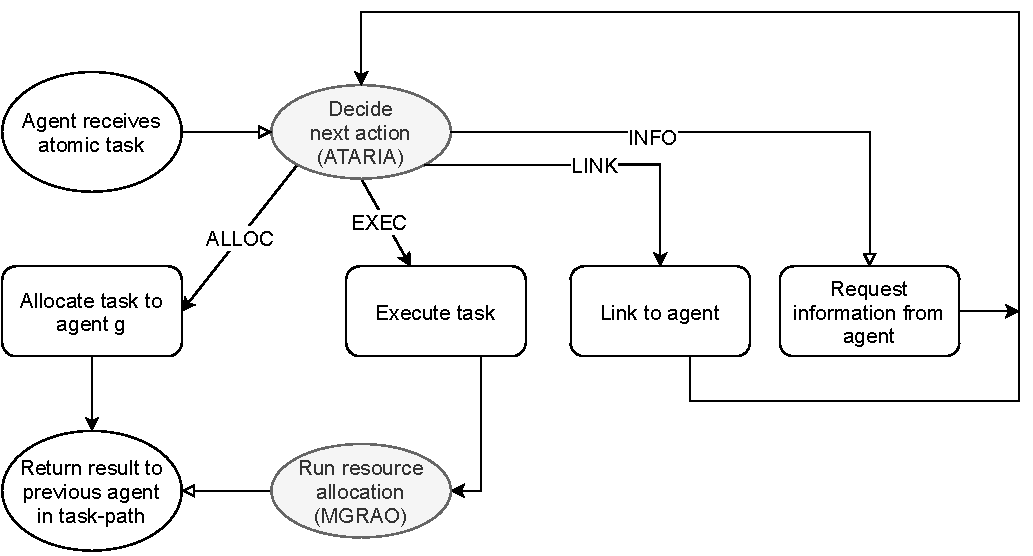
\includegraphics[width=0.9\linewidth,trim={25pt 0pt 25pt 0pt, clip}]{algorithm-flow-arc}
		\caption{Task-path agent flow}
		\label{fig:algorithm-flow-arc}
	\end{subfigure}
	\caption{\textbf{\acronymWSNOptimisation{}{} execution flowchart.} Shows how \acronymWSNOptimisation{}{} combines the \acronymATARIA{}{} and \acronymMGRAO{}{} algorithms and enables recursive allocation of tasks.}
	\label{fig:algorithm-flow}
\end{figure}
